\documentclass[11pt,twocolumn]{article}
\raggedbottom

% --- Codificación y lenguaje ---
\usepackage[T1]{fontenc}
\usepackage[utf8]{inputenc}
\usepackage[spanish]{babel}

% --- Matemática y fuentes ---
\usepackage{amsfonts, amssymb, amsthm}
\usepackage{amsmath}
\usepackage{derivative}

% --- Gráficos y tablas ---
\usepackage{graphicx}
\usepackage{animate}
\usepackage{caption}
\usepackage{subcaption}
\usepackage{booktabs}
\usepackage{ulem}
\usepackage{siunitx}

% --- Varios útiles ---
\usepackage[margin=2cm]{geometry}
\setlength{\emergencystretch}{3em}
\usepackage{enumitem}
\usepackage{csquotes}  % <- biblatex recomienda este paquete
\usepackage{cuted}
\usepackage{float}
\usepackage{placeins}
\usepackage{multirow}
\usepackage[dvipsnames]{xcolor}
\usepackage{tikz}
\usetikzlibrary{calc}

% --- Bibliografía ---
\usepackage[
  backend=biber,
  style=phys,      % puedes cambiar el estilo
  sorting=none
]{biblatex}
\addbibresource{literature.bib}
\AtBeginBibliography{\small\raggedright}

% --- Hipervínculos ---
\usepackage[
  colorlinks=true,
  linkcolor=Blue,
  urlcolor=Blue,
  citecolor=Blue,
  filecolor=Blue,
  pdfborder={0 0 0}
]{hyperref}

\begin{document}

% =====================================
% 0. Portada.
% =====================================
\begin{tikzpicture}[remember picture,overlay]
  \node[anchor=north east, inner sep=0pt]
    at ($(current page.north east)+(-1.8cm,-1.2cm)$)
    {
\includegraphics[height=2.8cm]{UdeC_logo_azul.png}};
\end{tikzpicture}

\begin{strip}
\begin{center}
\vspace*{-5\baselineskip}
{\Large \textbf{Universidad de Concepción}}\\[-2pt]
\small Facultad de Ciencias Físicas y Matemáticas\\[-2pt]
\small \textit{Física VII Introducción a la Mecánica Cuántica (510322-1)}\\[4pt]

{\Large \bfseries Informe 3: Efecto fotoeléctrico }\\
[2pt]
\small Profesor: Paulraj Manidurai\\[-2pt]
\small N. Ulloa C., J. Rosas S.\\[-2pt]
\small Concepción, Chile — 25 de noviembre de 2025
\end{center}
\hrule

% =====================================
% 1. Abstract.
% =====================================
\begin{center}
\begin{abstract}
En este informe se estudia el efecto fotoeléctrico utilizando una celda
fotoeléctrica iluminada con luz de distintos colores en la región visible.
Para cada configuración de la fuente luminosa (luz roja, verde y azul) se
mide el voltaje de frenado con la corriente de corte mínima manteniendo aproximadamente fija la intensidad de luz incidente. A partir de los pares $(f, V_0)$ obtenidos se ajusta una relación lineal $V_0(f)=mf+b$, de la
cual se estima una constante de Planck experimental
$h_{\text{exp}} \approx 2{,}3\times 10^{-34}\,\mathrm{J\,s}$ (cerca de un
34\% del valor de referencia) y una función trabajo efectiva del orden de
$0{,}5\,\mathrm{eV}$. Aunque la determinación cuantitativa presenta errores
sistemáticos significativos, los resultados reproducen cualitativamente que
el voltaje de corte crece al pasar de luz roja a azul, en concordancia con
la dependencia de la energía cinética máxima de los fotoelectrones con la
frecuencia y no con la intensidad de la radiación.
\end{abstract}
\end{center}


\noindent\rule{\textwidth}{0.4pt}\par\vspace{0.3cm}
\end{strip}

% ===========================
% 2. Objetivos.
% ===========================
\section{Objetivos.}

Los objetivos de esta experiencia son:

\begin{itemize}[leftmargin=*, itemsep=2pt, before=\sloppy, after=\fussy]
  \item A partir de los potenciales de corte medidos para luz roja, verde y azul, estimar la constante de Planck.
  \item Comparar las estimaciones con el valor de referencia y discutir la dependencia del potencial de corte y de la energía cinética máxima con la frecuencia de la radiación.
\end{itemize}

% ===========================
% 3. Marco teórico.
% ===========================
\section{Marco teórico.}

\subsection{Cuantización de la energía y constante de Planck}

El punto de partida de esta experiencia es la relación entre la energía de la radiación electromagnética y su frecuencia. A comienzos del siglo XX, Max Planck introdujo la idea de que los intercambios de energía entre la radiación y la materia ocurren en cuantos discretos de energía $E$ proporcionales a la frecuencia $f$ de la radiación \cite{planck1900_blackbody}:
\begin{equation*}
    E = h f,
\end{equation*}
donde $h$ es la constante de Planck. Esta hipótesis permitió explicar correctamente el espectro de la radiación de cuerpo negro y marcó el inicio de la teoría cuántica.

Dado que la frecuencia y la longitud de onda $\lambda$ están relacionadas por $f = c/\lambda$, con $c$ la rapidez de la luz en el vacío, la energía de un fotón también puede escribirse como
\begin{equation*}
    E = h f = h \frac{c}{\lambda}.
\end{equation*}
Esta expresión relaciona directamente la longitud de onda (o el color) de la luz con la energía de los fotones emitidos o absorbidos \cite{quantum_mechanics_photoelectric}.

\subsection{Efecto fotoeléctrico y relación \texorpdfstring{$eV_0 = hf - W$}{eV₀ = hf - W}}

En 1905, Albert Einstein aplicó la idea de cuantos de luz para explicar
el efecto fotoeléctrico, es decir, la emisión de electrones desde la
superficie de un metal iluminado con radiación de frecuencia
suficientemente alta \cite{einstein1905_photoelectric}. En este modelo,
la luz está compuesta por fotones, cada uno con energía
\begin{equation*}
    E_{\gamma} = h f,
\end{equation*}
donde $h$ es la constante de Planck y $f$ la frecuencia de la radiación.

Cuando un fotón es absorbido por un electrón en el metal, su energía se
reparte entre:
\begin{itemize}
  \item la energía necesaria para extraer al electrón del material,
        llamada función trabajo $W$ (o $\phi$), y
  \item la energía cinética con la que el electrón escapa.
\end{itemize}
Para los electrones emitidos con energía cinética máxima $K_{\max}$, el
balance de energía se escribe como
\begin{equation*}
    h f = K_{\max} + W.
\end{equation*}

En un montaje experimental típico se aplica entre el cátodo y el ánodo
un potencial de frenado (o potencial de corte) $V_0$, de tal manera que
los electrones emitidos deben ``subir'' una barrera de energía eléctrica
para llegar al ánodo. El valor de $V_0$ se define como aquel para el que
la corriente fotoeléctrica se anula: en ese caso, incluso los electrones
más energéticos son detenidos por el campo eléctrico. La energía
cinética máxima y el potencial de corte se relacionan entonces mediante
\begin{equation*}
    K_{\max} = e V_0,
\end{equation*}
donde $e$ es la carga del electrón. Sustituyendo en la ecuación anterior
se obtiene
\begin{equation*}
    e V_0 = h f - W,
\end{equation*}
es decir,
\begin{equation*}
    V_0(f) = \frac{h}{e}\,f - \frac{W}{e}.
\end{equation*}

Esta expresión muestra que el potencial de corte $V_0$ es una función
lineal de la frecuencia de la radiación incidente. Escribiendo
\begin{equation*}
    V_0(f) = m f + b,
\end{equation*}
se identifica la pendiente como
\begin{equation*}
    m = \frac{h}{e}
\end{equation*}
y el intercepto como
\begin{equation*}
    b = -\frac{W}{e} = \phi_0,
\end{equation*}
donde $\phi_0$ representa la contribución de la función trabajo (y, en
general, de posibles desplazamientos de referencia de potencial) en
unidades de voltaje. De este modo, midiendo $V_0$ para distintas
frecuencias $f$ y ajustando los datos experimentales a una recta de la
forma $V_0(f) = mf + b$, es posible estimar simultáneamente la constante
de Planck $h$ y una función trabajo efectiva $W$ a partir de
\begin{equation*}
    h_{\text{exp}} = e\,m,
    \qquad
    W_{\text{exp}} = -\,e\,b.
\end{equation*}

El análisis de datos consistirá
entonces en construir los pares $(f, V_0)$ para cada color y realizar un
ajuste por mínimos cuadrados a la recta
\begin{equation*}
    V_0(f) = m f + b,
\end{equation*}
de manera que la pendiente $m$ proporcione una estimación de
$\tfrac{h}{e}$ y el intercepto $b$ se interprete como
$\phi_0 = -\,W/e$.



% ===========================
% 4. Materiales:
% ===========================
\section{Materiales.}

Para llevar a cabo la experiencia se utilizaron los siguientes elementos:

\begin{itemize}
  \item Batería de 15 \text{V}.
  \item Fuente emisora de luz.
  \item Placas transparentes de color rojo, verde y azul.
  \item Resistencia de 1 \text{M $\Omega$}
  \item Potenciometro.
  \item Cables de conexión tipo banana.
  \item Multímetro digital para la medición de voltajes.
  \item Módulo fotoeléctrico.
\end{itemize}

% ===========================
% 5. Metodología.
% ===========================

\section{Metodología.}

El procedimiento seguido en la experiencia puede resumirse en los
siguientes pasos:

\begin{enumerate}
  \item Ensamblar el circuito tal como lo describe la figura~\ref{fig:circuito_detalle}. Y se dispone el módulo fotoeléctrico y la fuente emisora de luz tal como aparece en la figura~\ref{fig:montaje_experimental}.
  
  \item Se ajusta el potenciómetro tal que el voltaje medido en V sea cero, tal que se maximiza el voltaje de frenado y se maximiza la energía cinética de los electrones.

  \item Colocar una placa de algún color en la salida de la fuente lumínica apuntando al sensor del módulo de efecto fotoeléctrico.

  \item Medir el voltaje indicado por el voltímetro $V_0$.
  
  \item Repetir la medición del voltaje al menos cuatro veces para la misma placa, manteniendo las condiciones del montaje lo más constantes posible. Registrar todos los valores en una tabla.
  
  \item Repetir los pasos anteriores para los otras dos placas.
\end{enumerate}

En la Figura~\ref{fig:circuito_detalle} se presenta un diagrama esquemático
del circuito utilizado para la medición del voltaje relacionado a la energía cinética máxima (medido con el voltímetro $V_0$).
Por otra parte, en la Figura~\ref{fig:montaje_experimental}
se incluye una fotografía del montaje real sobre la mesa de trabajo, donde
se aprecia la disposición relativa entre el módulo fotoeléctrico y la fuente
luminosa. Ambas imágenes complementan la descripción del procedimiento
experimental descrito en esta sección.

\begin{figure}
    \centering
    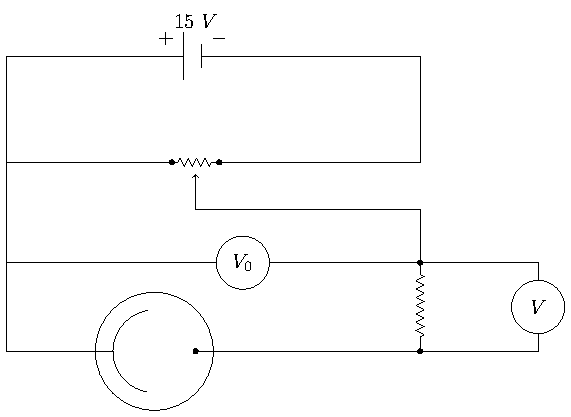
\includegraphics[width=0.9\linewidth]{img/montaje_completo.pdf}
    \caption{Diagrama esquemático del circuito utilizado para medir el voltaje
    relacionado a la energía cinética.}
    \label{fig:circuito_detalle}
\end{figure}

\begin{figure}
    \centering
    
\includegraphics[width=1\linewidth]{img/montaje.jpg}
    \caption{Fotografía del montaje experimental. Se observan el módulo
    fotoeléctrico y la unidad de iluminación enfrentados durante la toma
    de datos.}
    \label{fig:montaje_experimental}
\end{figure}


% ===========================
% 6. Resultados.
% ===========================

\section{Resultados.}

En esta experiencia se estudió la relación entre el potencial asociado a la corriente fotoeléctrica en una celda fotoeléctrica y la frecuencia de la luz incidente, con el objetivo de estimar la constante de Planck. 

Se trabajó con tres colores de luz en la región visible: rojo, verde y azul. Para cada color se registraron cuatro mediciones del voltaje $V_0$ (en milivolt) manteniendo fija la configuración del circuito y procurando que la intensidad de la fuente luminosa se mantuviera aproximadamente constante. Los voltajes medidos son reportados en el cuadro \ref{tab:voltajes}.
\begin{table}[ht]
    \centering
    \caption{Voltajes medidos para cada color de la luz incidente.}
    \begin{tabular}{lcccc}
        \hline
        \textbf{Color} & $V_1$ [mV] & $V_2$ [mV] & $V_3$ [mV] & $V_4$ [mV] \\
        \hline
        Rojo  & $101.3$ & $95.1$  & $96.6$  & $77.4$  \\
        Verde & $287.8$ & $289.0$ & $287.9$ & $290.0$ \\
        Azul  & $377.5$ & $372.0$ & $370.0$ & $368.0$ \\
        \hline
    \end{tabular}
    \label{tab:voltajes}
\end{table}
A cada color se le asoció una longitud de onda nominal de la luz incidente, representativa de la región roja, verde y azul del espectro visible:
\begin{align*}
    \lambda_R &\approx 688\,\mathrm{nm},\\[2pt]
    \lambda_V &\approx 533\,\mathrm{nm},\\[2pt]
    \lambda_A &\approx 473\,\mathrm{nm}.
\end{align*}
A partir de estas longitudes de onda se calcularon las frecuencias mediante la relación $f = c/\lambda$, donde $c$ es la rapidez de la luz en el vacío.

% ===========================
% 7. Análisis de datos. 
% ===========================
\section{Análisis de datos.}

\subsection{Tratamiento de los datos experimentales}

Para cada color de la luz incidente (rojo, verde y azul) se
registraron cuatro mediciones del voltaje $V_0$ en el circuito, en
milivolt, manteniendo fija la configuración de la celda
fotoeléctrica y de la fuente luminosa. A partir de estos datos se
calculó, para cada color $i$, el voltaje promedio $\overline{V_0}_i$
y su desviación estándar $\sigma_{V_0,i}$ mediante
\begin{align*}
    \overline{V}_i &= \frac{1}{N}\sum_{k=1}^{N} V_{i,k},
    \\[4pt]
    \sigma_{V_i} &= \sqrt{\frac{1}{N-1}
      \sum_{k=1}^{N} \bigl(V_{i,k} - \overline{V}_i\bigr)^2},
\end{align*}
con $N = 4$ el número de mediciones por color. Como los datos se
obtuvieron en milivolt, los promedios y desviaciones estándar se
convirtieron luego a volt multiplicando por $10^{-3}$.

Los valores obtenidos fueron, aproximadamente,
\begin{align*}
    \overline{V_0}_{\text{rojo}} &\approx 0{,}093 \pm 0{,}010~\text{V},\\
    \overline{V_0}_{\text{verde}} &\approx 0{,}281 \pm 0{,}008~\text{V},\\
    \overline{V_0}_{\text{azul}} &\approx 0{,}372 \pm 0{,}004~\text{V}.
\end{align*}

A cada color se le asoció una longitud de onda nominal $\lambda_i$
de la luz incidente, representativa de la región roja, verde y azul
del espectro visible. En este análisis se utilizaron los valores
\begin{align*}
    \lambda_R &= 688~\text{nm}, \\[4pt]
    \lambda_V &= 533~\text{nm}, \\[4pt]
    \lambda_A &= 473~\text{nm},
\end{align*}
a partir de los cuales se calcularon las frecuencias correspondientes
mediante
\begin{equation*}
    f_i = \frac{c}{\lambda_i},
\end{equation*}
con $c = 2{,}9979\times 10^{8}\,\text{m/s}$ la rapidez de la luz en el
vacío. De este modo se obtuvieron, en orden rojo–verde–azul,
\begin{align*}
    f_R &\approx 4{,}36\times 10^{14}~\text{Hz},\\[4pt]
    f_V &\approx 5{,}63\times 10^{14}~\text{Hz},\\[4pt]
    f_A &\approx 6{,}34\times 10^{14}~\text{Hz}.
\end{align*}
Estos tres pares experimentales $(f_i, \overline{V_0}_i)$, con sus
respectivas barras de error en voltaje, constituyen la base del
ajuste lineal $V_0(f)$.

Siguiendo la ecuación de Einstein para el efecto fotoeléctrico,
\begin{equation*}
    eV_0 = hf - W,
\end{equation*}
el potencial de frenado $V_0$ y la frecuencia $f$ se relacionan, para
un mismo material (función trabajo $W$ constante), como
\begin{equation*}
    V_0(f) = \frac{h}{e}\,f - \frac{W}{e}.
\end{equation*}
Es decir, se espera una relación lineal entre el voltaje y la
frecuencia de la forma
\begin{equation*}
    V(f) = m f + b,
\end{equation*}
con
\begin{equation*}
    m = \frac{h}{e},
    \qquad
    b = -\,\frac{W}{e}.
\end{equation*}

Con los tres puntos
experimentales $(f_i,\overline{V_0}_i)$ se realizó un ajuste por
mínimos cuadrados a la recta $V_0(f) = m f + b$, utilizando
\href{https://udeconce-my.sharepoint.com/:u:/g/personal/jrosas2022_udec_cl/IQAlghGK5KtVSIMtoxaivDERAXu_a-6XY6fiqCMTyiOVOwg?e=nkgkxH}{este script de Python}
(\texttt{analisis\_leds\_planck.py}). El ajuste entregó los valores
\begin{align*}
    m &\approx 1{,}42\times 10^{-15}~\text{V/Hz},
    \\[4pt]
    b &\approx -5{,}23\times 10^{-1}~\text{V}.
\end{align*}

A partir de la pendiente se obtuvo la estimación experimental de la
constante de Planck,
\begin{equation*}
    h_{\text{exp}} = e\,m \approx 2{,}27\times 10^{-34}~\text{J·s},
\end{equation*}
lo que corresponde a aproximadamente un $34\%$ del valor de
referencia
\begin{equation*}
    h_{\text{ref}} = 6{,}63\times 10^{-34}~\text{J·s},
\end{equation*}
es decir, un error relativo del orden de un $66\%$. Por otra parte,
a partir del intercepto se estimó una función trabajo efectiva
\begin{equation*}
    W_{\text{exp}} = -\,e\,b \approx 8{,}4\times 10^{-20}~\text{J}
    \approx 0{,}52~\text{eV}.
\end{equation*}
Este valor es del orden de fracciones de eV, menor que las funciones
trabajo típicas de metales puros (del orden de unos pocos eV), lo que
indica que el montaje real y la interpretación del voltaje medido
incluyen contribuciones adicionales (por ejemplo, las condiciones del ambiente de medición o la electrónica interna
del módulo) que se discuten más adelante.

El procedimiento completo (cálculo de promedios, desviaciones
estándar, frecuencias y ajuste lineal $V_0(f)$) se implementó en el
script ya mencionado en \texttt{Python}. La Figura~\ref{fig:grafico_V_vs_f}
muestra los puntos experimentales $(f_i,\overline{V_0}_i)$ con sus
barras de error y la recta ajustada a partir de estos datos,
generada mediante el script
\href{https://udeconce-my.sharepoint.com/:u:/g/personal/jrosas2022_udec_cl/IQC8_r32rtReTb8lnTCGmHhyASGzSxLxzgiaxr_dnAOnC3M?e=oXf11t}{\texttt{grafico\_V\_vs\_f.py}}.

\begin{figure}[ht]
    \centering
    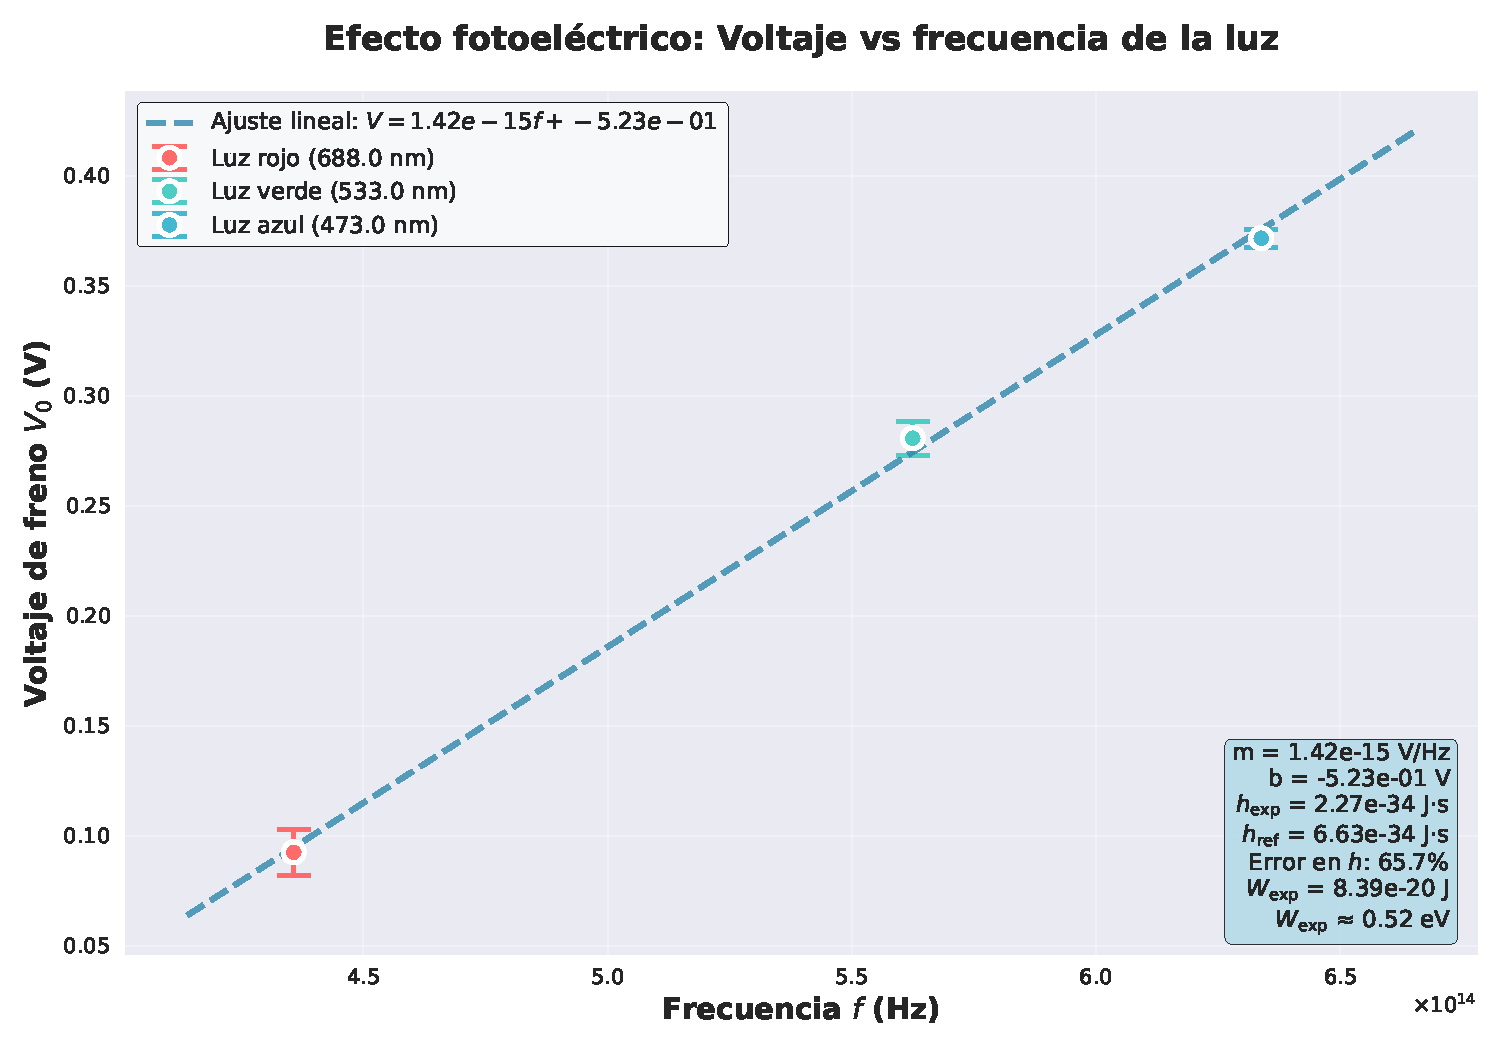
\includegraphics[width=1\linewidth]{img/grafico_V_vs_f.pdf}
    \caption{Voltaje de freno promedio medido en el circuito en función
    de la frecuencia de la luz incidente sobre la celda fotoeléctrica.
    Cada punto corresponde a un color (rojo, verde y azul) y las barras
    de error representan la desviación estándar de las cuatro
    mediciones de voltaje para cada caso. La recta ajustada
    $V_0(f) = mf + b$ presenta una pendiente
    $m \approx 1{,}42\times 10^{-15}~\text{V/Hz}$ e intercepto
    $b \approx -5{,}23\times 10^{-1}~\text{V}$, a partir de los cuales
    se obtiene una estimación de la constante de Planck
    $h_{\text{exp}} \approx 2{,}27\times 10^{-34}~\text{J·s}$ y de una
    función trabajo efectiva $W_{\text{exp}} \approx 0{,}52~\text{eV}$.}
    \label{fig:grafico_V_vs_f}
\end{figure}

\subsection{¿Depende el potencial de corte de la intensidad de la luz o del color?}

En el efecto fotoeléctrico estándar, el potencial de corte $V_0$ se
define como el voltaje retardador que reduce a cero la corriente
fotoeléctrica. La ecuación de Einstein permite escribir
\begin{equation*}
    eV_0 = K_{\max} = hf - W,
\end{equation*}
donde $W$ es la función trabajo del material. De esta expresión se
concluye de forma explícita que, para un mismo material ($W$
constante):

\begin{itemize}
  \item El potencial de corte no depende de la intensidad de la luz.
  Aumentar la intensidad sólo incrementa el número de electrones
  emitidos (la corriente), pero no cambia la energía cinética máxima
  de cada electrón, por lo que el valor de $V_0$ necesario para
  frenarlos sigue siendo el mismo.
  \item El potencial de corte sí depende del color (frecuencia) de la luz.
  Al aumentar $f$, la energía del fotón $hf$ aumenta y, en
  consecuencia, la energía cinética máxima $K_{\max}$ crece, lo que
  exige un potencial de corte mayor para anular la corriente.
\end{itemize}

En el presente experimento no se varió sistemáticamente la intensidad
de la luz, por lo que no es posible estudiar de manera directa su
efecto sobre el potencial de corte. Sin embargo, sí se trabajó con
tres colores distintos de la radiación incidente (rojo, verde y
azul), para los cuales se obtuvieron los voltajes promedio
\begin{equation*}
    \overline{V}_{\text{rojo}} < \overline{V}_{\text{verde}} <
    \overline{V}_{\text{azul}},
\end{equation*}
en correspondencia con el aumento de frecuencia desde el rojo hacia
el azul. Esta jerarquía es coherente con la situación fotoeléctrica
ideal: el voltaje efectivo asociado al corte de la corriente no debe
depender de la intensidad, pero sí del color (frecuencia) de
la radiación incidente.

\subsection[¿Depende la energía cinética máxima del potencial de corte o del color?]{¿Depende la energía cinética máxima de los electrones de \texorpdfstring{$V_0$}{V0} o del color?}

En el marco del efecto fotoeléctrico, la energía cinética máxima de
los electrones emitidos se puede expresar de dos maneras equivalentes:
\begin{equation*}
    K_{\max} = hf - W
    \qquad \text{y} \qquad
    K_{\max} = eV_0.
\end{equation*}
Desde un punto de vista \textbf{matemático}, la segunda relación
muestra que $K_{\max}$ es proporcional al potencial de corte $V_0$.
Sin embargo, físicamente la \textbf{causa} de la variación de
$K_{\max}$ es el \textbf{color} de la luz, es decir, su frecuencia
$f$:

\begin{itemize}
  \item Al cambiar el color (variar $f$), cambia la energía del fotón
        $hf$ y, por tanto, cambia $K_{\max}$.
  \item El potencial de corte $V_0$ se ajusta precisamente para
        anular la contribución de esos electrones más energéticos;
        por eso $K_{\max} = eV_0$ es una forma de medir
        experimentalmente la energía, no su causa.
\end{itemize}

El análisis de la sección anterior
muestra que los puntos $(f_i,\overline{V_0}_i)$ siguen aproximadamente
una recta creciente en $f$, de modo que tanto $V_0$ como $K_{\max} =
eV$ aumentan al pasar de luz roja a verde y luego a azul. De esta
forma, los resultados obtenidos son coherentes con la predicción
teórica de que es la \textbf{frecuencia} (y no la intensidad) de la
luz la que determina la energía cinética máxima de los electrones
emitidos en el efecto fotoeléctrico.


% ===========================
% 8. Discusión. 
% ===========================
\section{Discusión.}

A partir de los voltajes registrados para las tres configuraciones de la
fuente luminosa (luz roja, verde y azul) y de las frecuencias asociadas
a cada longitud de onda nominal, se obtuvo un ajuste lineal de la forma
$V(f) = mf + b$ con
\begin{align*}
    m \approx 1{,}42\times 10^{-15}~\text{V/Hz},
    \\[4pt]
    b \approx -5{,}23\times 10^{-1}~\text{V}.
\end{align*}
A partir de la pendiente se estimó la constante de Planck experimental
como
\begin{equation*}
    h_{\text{exp}} = e\,m \approx 2{,}27\times 10^{-34}~\text{J\,s},
\end{equation*}
lo que corresponde a aproximadamente un $34\%$ del valor de referencia
\begin{equation*}
    h_{\text{ref}} \approx 6{,}63\times 10^{-34}~\text{J\,s},
\end{equation*}
es decir, un error relativo del orden de un $66\%$. El intercepto
negativo se traduce en una función trabajo efectiva
\begin{equation*}
    W_{\text{exp}} = -\,e\,b \approx 8{,}4\times 10^{-20}~\text{J}
    \approx 0{,}52~\text{eV}.
\end{equation*}
Este valor es del orden de fracciones de eV, significativamente menor
que las funciones trabajo típicas de metales puros (del orden de unos
pocos eV), lo que sugiere que $W_{\text{exp}}$ debe interpretarse como
un parámetro efectivo que incluye no sólo la función trabajo del
material fotosensible, sino también contribuciones de la electrónica
interna del módulo y del esquema de medición.

La comparación entre el valor de $h_{\text{exp}}$ y $h_{\text{ref}}$
indica claramente que el error dominante no es de tipo estadístico,
sino sistemático. Entre las principales fuentes de error sistemático se
pueden mencionar:

\begin{itemize}
  \item \textbf{Interpretación del voltaje medido.} El voltímetro está
        conectado en un circuito que incluye la celda fotoeléctrica, una
        resistencia de $1\,\text{M}\Omega$ y posiblemente otros elementos
        internos del módulo. El voltaje leído no coincide de manera
        estricta con el potencial de corte ideal $V_0$ de la ecuación de
        Einstein, sino con una combinación de caídas de tensión en el
        circuito. Cualquier diferencia entre el voltaje medido y el
        verdadero potencial de corte se traduce en un sesgo en la
        pendiente $m$ y, por tanto, en $h_{\text{exp}}$.

    \item {La alta luminosidad del ambiente.} Al momento de realizar las mediciones, si bien estaba presente la protección, igualmente la luminosidad de los focos del laboratorio pudieron haber tenido alguna interferencia en la producción de corriente, lo que pudo haber entorpecido la recolección de datos.

  \item \textbf{Uso de longitudes de onda nominales.} Las longitudes de
        onda empleadas corresponden a valores nominales para luz roja,
        verde y azul, no a una medición espectral directa de la fuente
        luminosa y de las placas de color utilizadas. El espectro real
        puede ser relativamente ancho y no estar centrado exactamente en
        los valores de $\lambda$ adoptados, lo que introduce una
        incertidumbre en las frecuencias $f_i$ y afecta la recta ajustada.

  \item \textbf{Número reducido de puntos y linealidad.} El ajuste
        lineal se realizó a partir de sólo tres puntos experimentales,
        de modo que pequeñas variaciones en los voltajes o en las
        frecuencias asociadas pueden producir cambios apreciables en la
        pendiente y en el intercepto. Además, cualquier desviación de la
        relación idealmente lineal $V_0(f)$ (debida, por ejemplo, a
        respuestas no lineales del módulo) no puede ser detectada ni
        corregida con tan pocos puntos.

\end{itemize}

A pesar de estas limitaciones cuantitativas, el experimento reproduce de
forma cualitativa las dependencias fundamentales del efecto
fotoeléctrico. La ecuación de Einstein,
\begin{equation*}
    eV_0 = K_{\max} = hf - W,
\end{equation*}
muestra que, para un material dado (función trabajo fija), el potencial
de corte $V_0$ es independiente de la intensidad de la luz incidente y
depende únicamente de su frecuencia. Aumentar la intensidad aumenta la
corriente fotoeléctrica (número de electrones emitidos por segundo), pero
no modifica la energía cinética máxima de cada electrón, de modo que el
valor de $V_0$ permanece inalterado. En cambio, al pasar de luz roja a
verde y luego a azul, la frecuencia $f$ aumenta, la energía de los
fotones $hf$ crece y, en consecuencia, se requiere un potencial de corte
mayor para anular la corriente.

Los datos experimentales son coherentes con este comportamiento: los
voltajes efectivos promedio satisfacen
\begin{equation*}
    \overline{V_0}_{\text{rojo}} < \overline{V_0}_{\text{verde}} <
    \overline{V_0}_{\text{azul}},
\end{equation*}
en paralelo con el aumento de frecuencia de la radiación incidente. De
este modo, aunque la estimación de $h$ presenta un error sistemático
importante y la función trabajo efectiva difiere de los valores
esperados para un metal ideal, la experiencia permite verificar
cualitativamente que es el \textbf{color} (frecuencia) de la luz, y no
su intensidad, el que controla la energía cinética máxima de los
electrones emitidos.

% ===========================
% 9. Conclusiones.
% ===========================
\section{Conclusiones.}

A partir del trabajo realizado se pueden extraer las siguientes
conclusiones principales:

\begin{itemize}
  \item Los voltajes efectivos medidos para las tres configuraciones de
        la fuente luminosa (luz roja, verde y azul) muestran una
        tendencia creciente con la frecuencia de la luz incidente, es
        decir,
        \[
            \overline{V_0}_{\text{rojo}} < \overline{V_0}_{\text{verde}} <
            \overline{V_0}_{\text{azul}}.
        \]
        Esta jerarquía es cualitativamente consistente con la expresión
        $E = hf$ para la energía de los fotones y con la relación
        lineal $V_0(f) = \tfrac{h}{e}f - \tfrac{W}{e}$ predicha por el
        modelo de Einstein para el efecto fotoeléctrico.

  \item En el efecto fotoeléctrico ideal, el potencial de corte $V_0$
        resulta \textbf{independiente de la intensidad} de la luz
        incidente y \textbf{dependiente sólo de la frecuencia} (color),
        ya que la energía cinética máxima viene dada por
        $K_{\max} = hf - W$. Aunque en este montaje no se estudió
        de forma sistemática la variación con la intensidad, los
        resultados obtenidos son coherentes con esta predicción: los
        cambios observados en el voltaje efectivo se asocian a cambios
        de color, no a variaciones controladas de brillo.

  \item A partir del ajuste lineal $V_0(f) = mf + b$ se obtuvo una
        estimación experimental de la constante de Planck
        $h_{\text{exp}} \approx 2{,}27\times 10^{-34}~\text{J\,s}$,
        que representa aproximadamente un $34\%$ del valor de
        referencia $h_{\text{ref}} \approx 6{,}63\times 10^{-34}~\text{J\,s}$.
        El error relativo, del orden de un $66\%$, se atribuye
        principalmente a errores sistemáticos asociados a la
        interpretación del voltaje medido como potencial de corte ideal,
        al uso de longitudes de onda nominales y al número reducido de
        puntos en el ajuste.

  \item El mismo ajuste permite estimar una función trabajo efectiva
        $W_{\text{exp}} \approx 0{,}52~\text{eV}$, valor inferior al
        esperado para metales típicos. Esta discrepancia sugiere que
        $W_{\text{exp}}$ incorpora no sólo la función trabajo del
        material fotosensible, sino también efectos instrumentales y
        detalles del módulo fotoeléctrico empleado.

  \item A pesar de las discrepancias cuantitativas en la determinación
        de $h$ y de $W$, la experiencia cumple su objetivo principal:
        ilustrar de manera cualitativa la relación entre energía y
        frecuencia en el efecto fotoeléctrico. El hecho de que el
        voltaje necesario para “frenar” a los electrones aumente al
        pasar de luz roja a azul refleja directamente que la energía
        cinética máxima de los fotoelectrones está controlada por la
        frecuencia de la luz incidente, núcleo de la explicación
        cuántica propuesta por Einstein.
\end{itemize}



% ===========================
% 10. Referencias.
% ===========================

\begingroup
\raggedright
\sloppy
\printbibliography
\endgroup

\end{document}
